\documentclass[12pt,a4paper]{article}

\usepackage[utf8]{inputenc}
\usepackage[T1]{fontenc}
\usepackage{times}
\usepackage[margin=2.5cm]{geometry}
\usepackage{amsmath,amssymb}
\usepackage{graphicx}
\usepackage{booktabs}
\usepackage{enumitem}
\usepackage{algorithm}
\usepackage{algpseudocode}
\usepackage{hyperref}
\usepackage{listings}
\usepackage{xcolor}
\usepackage{caption}
\usepackage{subcaption}
\usepackage{float}

\hypersetup{colorlinks=true,linkcolor=blue,citecolor=blue,urlcolor=blue}

\graphicspath{{figures/}}

\lstset{
  basicstyle=\ttfamily\small,
  keywordstyle=\color{blue}\bfseries,
  commentstyle=\color{gray},
  frame=single,
  breaklines=true
}

\title{
  \textbf{ASSIGNMENT 2} \\[0.5em]
  \Large Advancing Front Hole Filling on 3D Meshes
}
\author{}
\date{}

\begin{document}
\maketitle

\noindent\textbf{Member:} \\
Truong Tri Dung -- MITIU25208 \\
To Thanh Thuyen -- MITIU25207 \\
Nguyen Thanh Nghia -- MITIU25205

\vspace{1em}

% ============================================================
\section{Introduction}
% ============================================================

Hole filling is a fundamental problem in 3D mesh processing. Holes commonly arise during 3D scanning due to occlusion, sensor noise, or reflective surfaces. This assignment implements the \textbf{Advancing Front} method as a MeshLab C++ filter plugin to fill holes in triangle meshes.

The Advancing Front method was first introduced in the context of unstructured mesh generation \cite{lo1985} and later adapted for hole filling by Liepa \cite{liepa2003} and Zhao et al.\ \cite{zhao2007}. The core idea is to progressively grow new triangles from the hole boundary inward, selecting vertices by their local angle and applying geometric rules to produce well-shaped triangles that conform to the surrounding mesh structure.

% ============================================================
\section{Algorithm}
% ============================================================

The algorithm operates in three stages: hole detection, advancing front triangulation, and post-processing smoothing.

% ------------------------------------------------------------
\subsection{Hole Detection}
% ------------------------------------------------------------

A \textbf{boundary edge} is an edge that belongs to exactly one triangle. A \textbf{hole} is a closed loop of boundary edges.

\begin{enumerate}[leftmargin=2em]
  \item Compute face--face adjacency for the entire mesh.
  \item Mark each face edge as \emph{border} if it has no adjacent face on that side.
  \item Mark each vertex as \emph{border} if it belongs to at least one border edge.
  \item Starting from any unvisited border edge $(v_i, v_j)$, trace the boundary loop: from $v_j$, find the next border edge leaving $v_j$ that differs from the incoming edge. Continue until the loop closes back to $v_i$.
  \item Record the ordered vertex indices, 3D positions, and per-vertex normals. Discard loops exceeding the \texttt{MaxHoleSize} threshold.
\end{enumerate}

The tracing uses VCG's vertex--face iterator to enumerate all faces around the current vertex and locate the next border edge, ensuring correct traversal even for complex boundary configurations.

\subsubsection{Visualizing Hole Boundaries}

To assist with hole detection and visualization, the plugin includes a dedicated filter that highlights hole boundaries. This feature can be accessed via:

\begin{center}
\texttt{Filters > Selection > Detect Hole Boundary (Red)}
\end{center}

This filter automatically identifies all boundary vertices that form holes in the mesh and colors them red (RGB: 255, 0, 0) for easy visualization. The implementation iterates through all vertices and marks those flagged as boundary vertices (\texttt{IsB()}) with red color. This visualization step is particularly useful for:

\begin{itemize}[leftmargin=2em]
  \item Verifying that holes have been correctly detected
  \item Assessing the size and complexity of holes before filling
  \item Identifying multiple holes in a single mesh
  \item Confirming that the hole boundary forms a valid closed loop
\end{itemize}

\begin{figure}[H]
\centering
\begin{subfigure}[b]{0.48\textwidth}
  \centering
  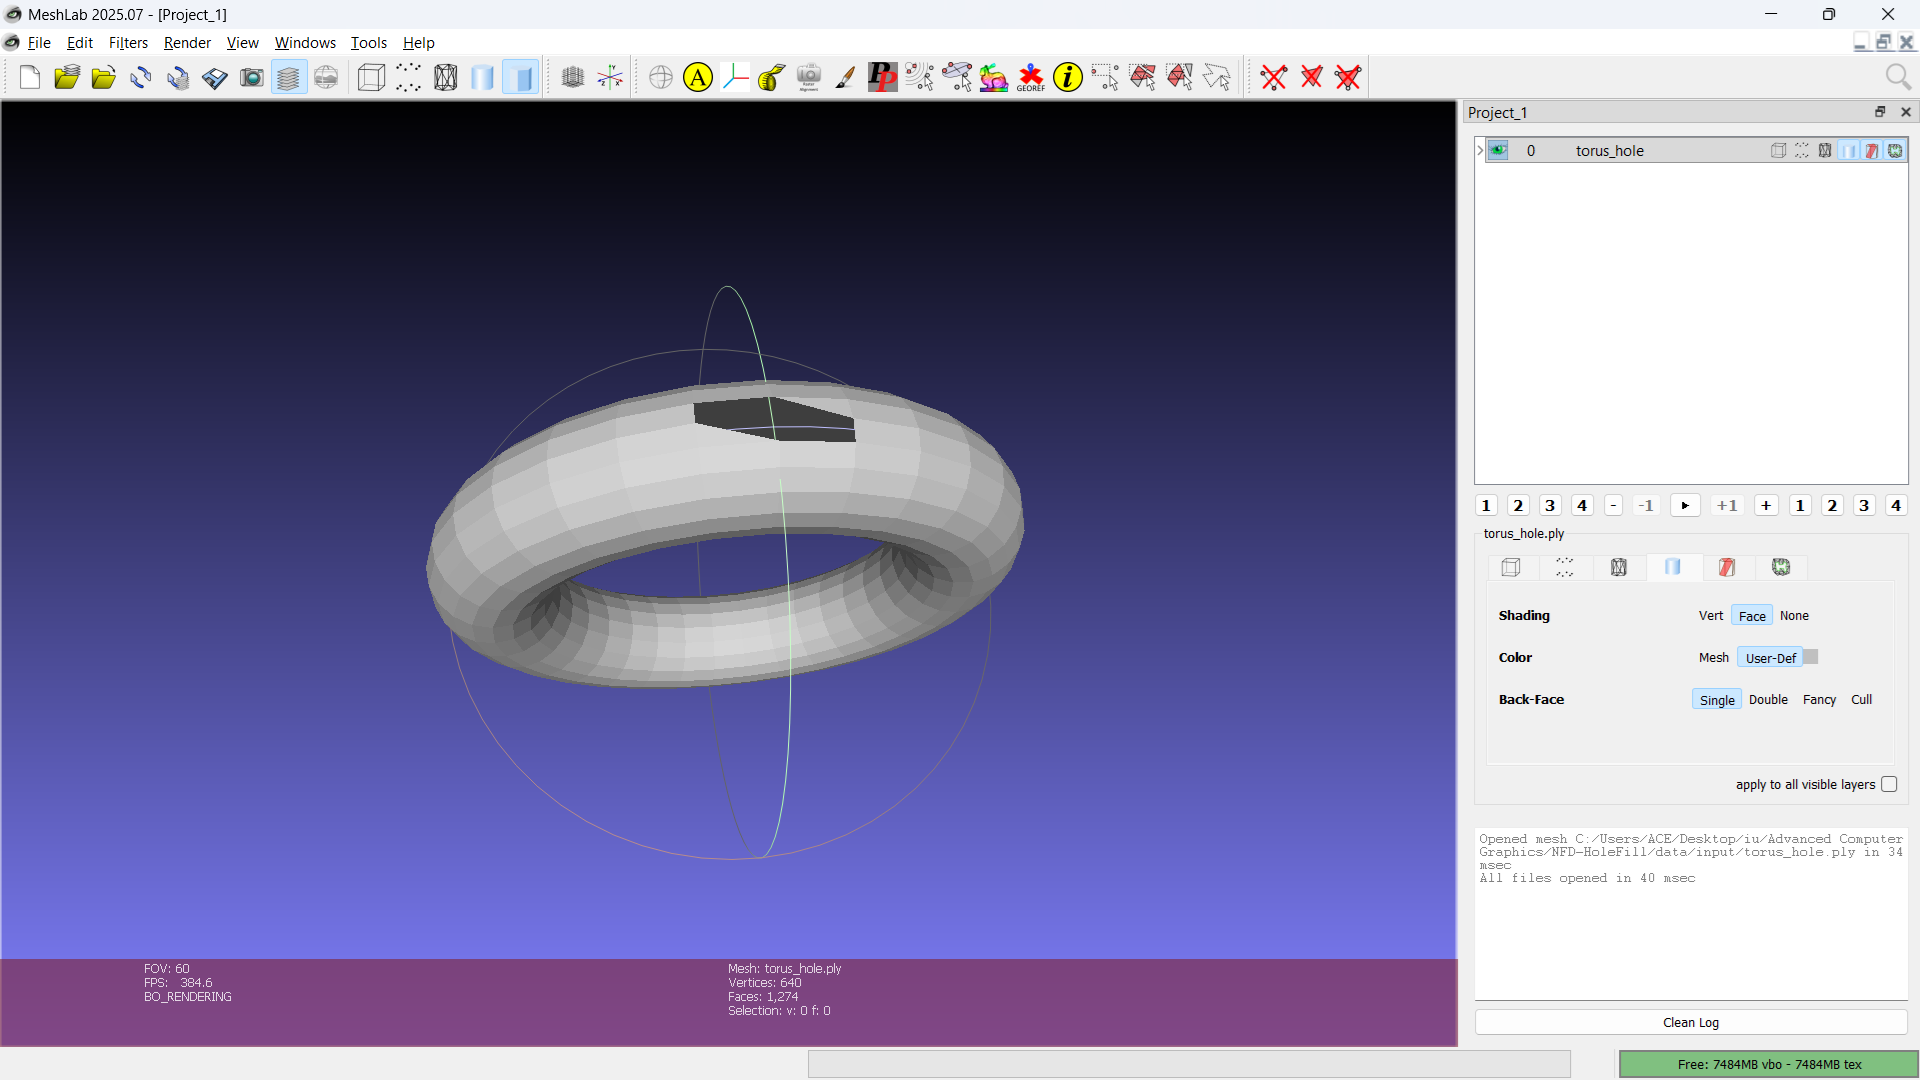
\includegraphics[width=\textwidth]{01_torus_with_hole.png}
  \caption{Torus mesh with a hole}
  \label{fig:torus_overview}
\end{subfigure}
\hfill
\begin{subfigure}[b]{0.48\textwidth}
  \centering
  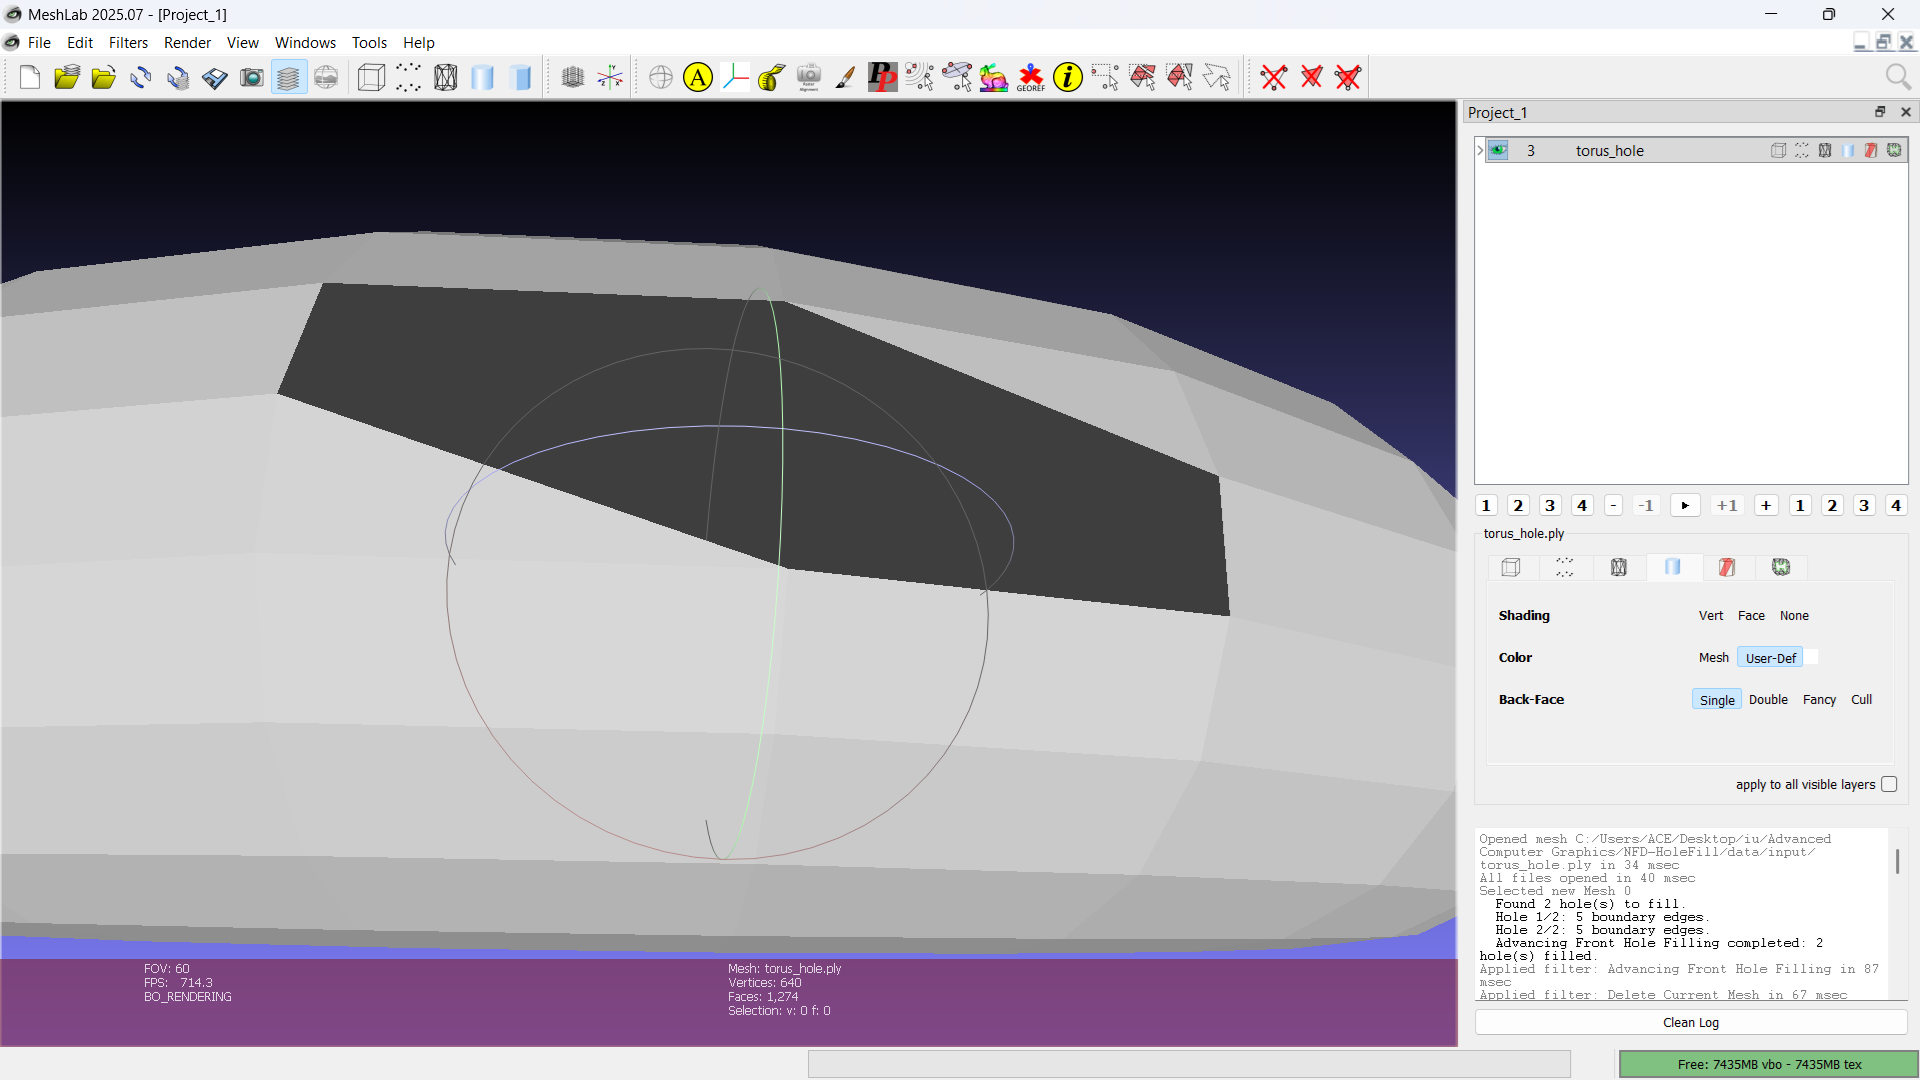
\includegraphics[width=\textwidth]{02_torus_closeup.png}
  \caption{Close-up of the hole boundary}
  \label{fig:torus_closeup}
\end{subfigure}
\caption{Hole detection on a torus mesh. The boundary edges form a closed loop around the missing region.}
\label{fig:torus_hole}
\end{figure}

\begin{figure}[H]
\centering
\begin{subfigure}[b]{0.48\textwidth}
  \centering
  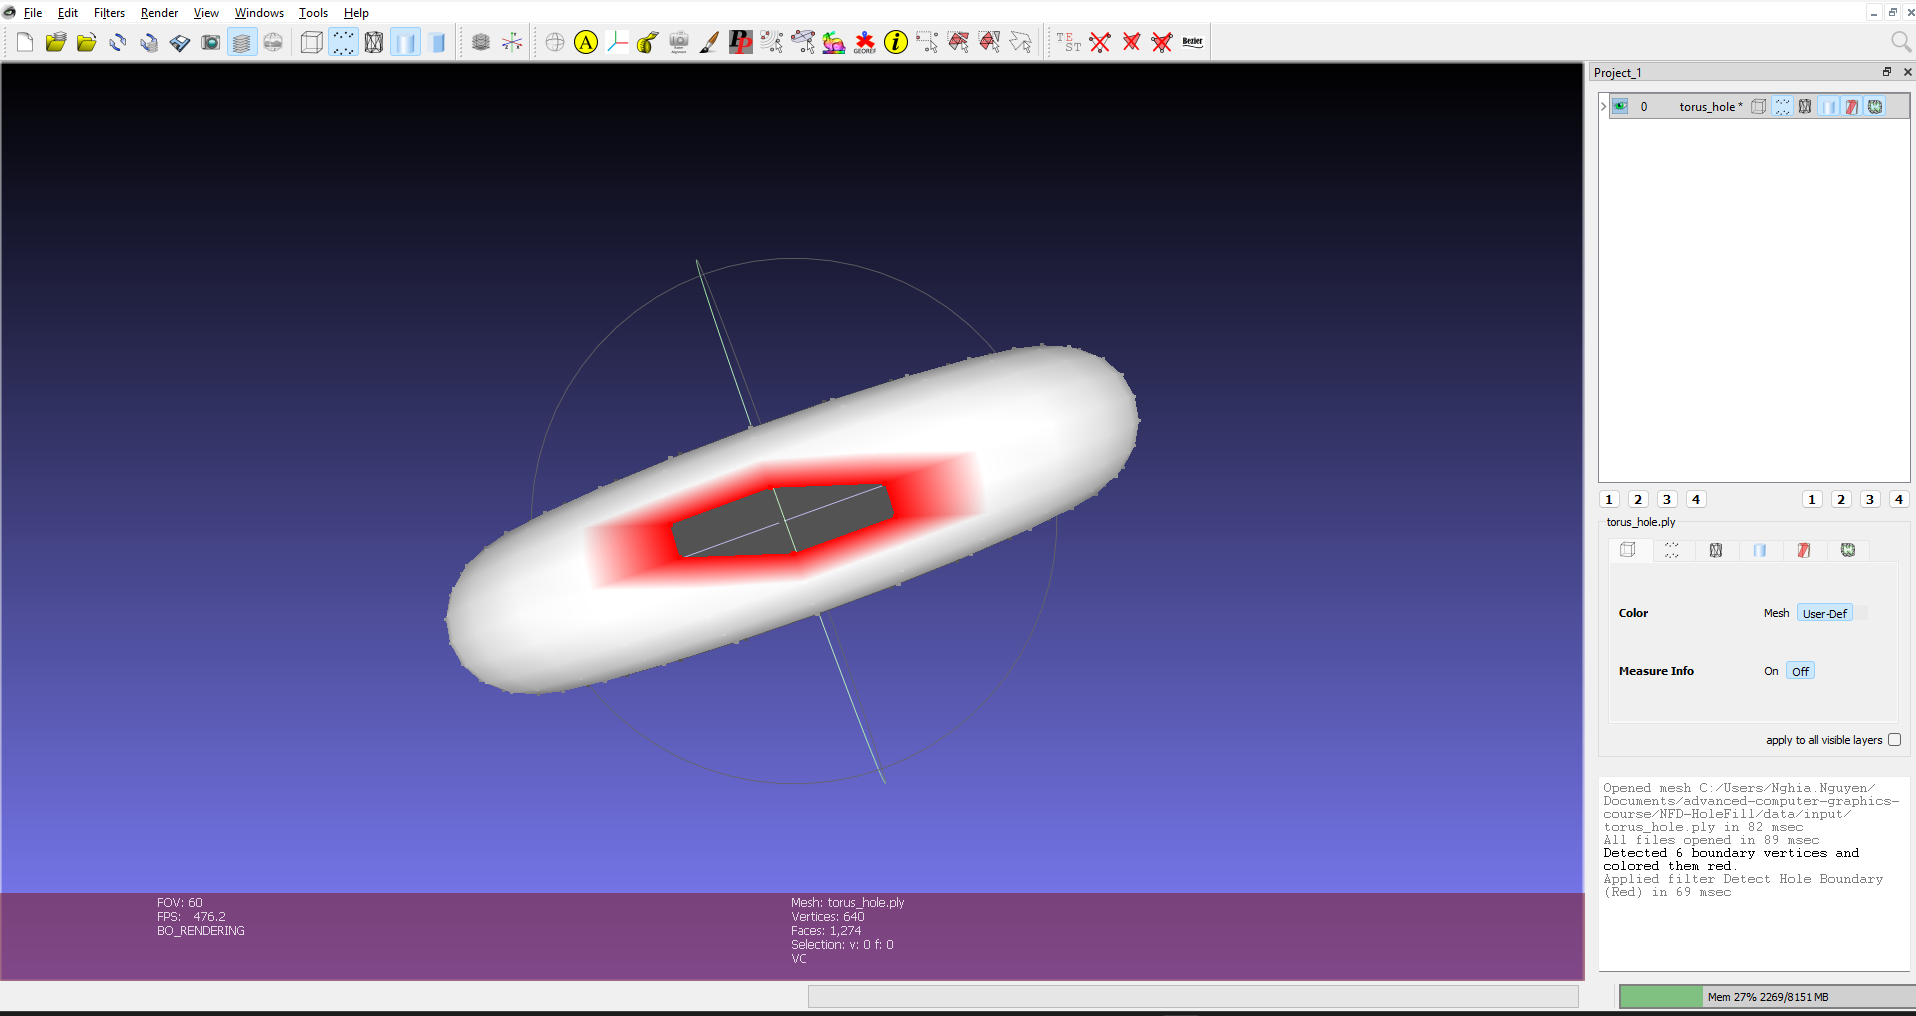
\includegraphics[width=\textwidth]{08_boundary_detection_red_vert_view.png}
  \caption{Overview of boundary detection}
  \label{fig:boundary_overview}
\end{subfigure}
\hfill
\begin{subfigure}[b]{0.48\textwidth}
  \centering
  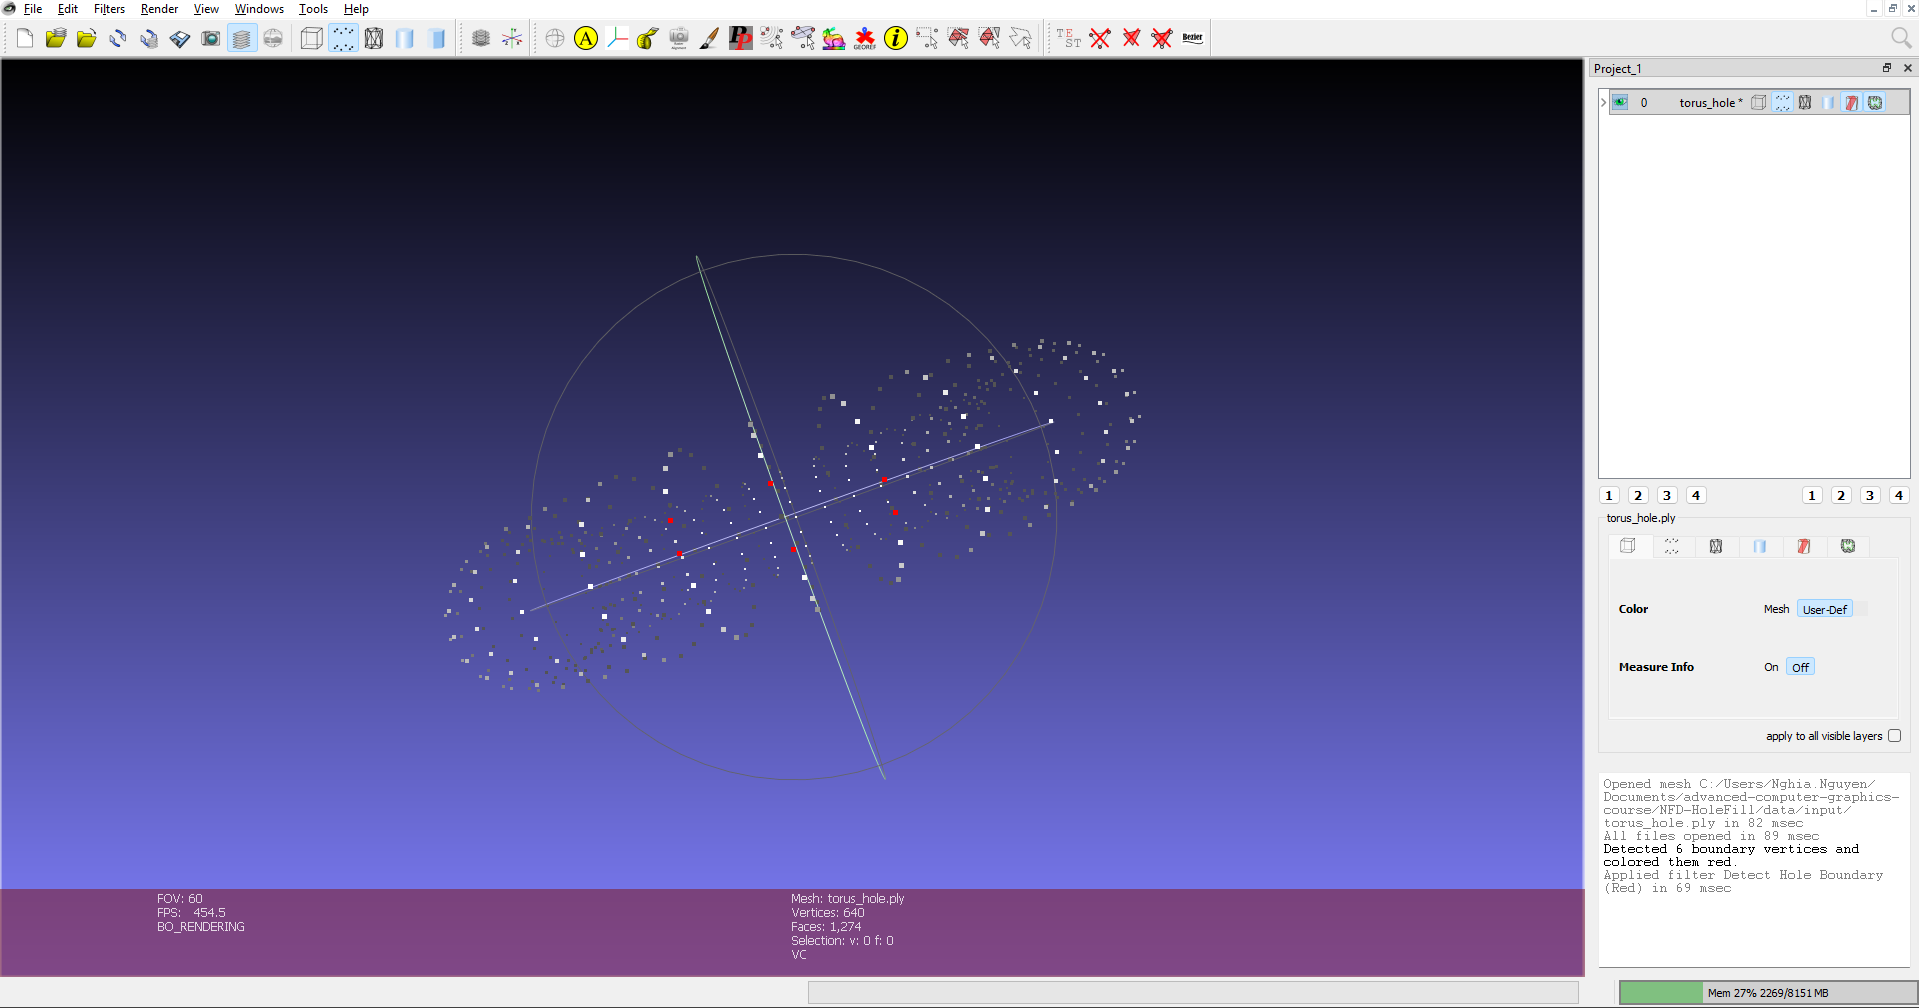
\includegraphics[width=\textwidth]{08_boundary_detection_red_vert_points.png}
  \caption{Close-up of red boundary vertices}
  \label{fig:boundary_closeup}
\end{subfigure}
\caption{Boundary vertices highlighted in red using the \texttt{Detect Hole Boundary (Red)} filter. All boundary vertices are colored with RGB(255, 0, 0) for easy visualization before applying the hole filling algorithm.}
\label{fig:boundary_detection}
\end{figure}

% ------------------------------------------------------------
\subsection{Advancing Front Triangulation}
% ------------------------------------------------------------

The advancing front is initialized as the boundary loop. At each iteration, the front vertex with the smallest interior angle is selected and one of three rules is applied. The process continues until only three vertices remain, which form the final closing triangle.

\subsubsection{Angle Computation}

For each vertex $v_i$ on the active front, the interior angle $\theta_i$ is computed between its two adjacent front edges:
\begin{align}
  \mathbf{e}_1 &= v_{i-1} - v_i, \qquad \mathbf{e}_2 = v_{i+1} - v_i \\[4pt]
  \cos\theta_i &= \frac{\mathbf{e}_1 \cdot \mathbf{e}_2}{\|\mathbf{e}_1\| \cdot \|\mathbf{e}_2\|} \\[4pt]
  \theta_i &= \arccos(\cos\theta_i)
\end{align}

The vertex $v_{\min}$ with the smallest angle $\theta_{\min}$ is selected for processing. Selecting the smallest angle first ensures that narrow gaps are closed before wide ones, producing more uniform triangles and preventing self-intersection.

% ── Rule 1 ──
\subsubsection{Rule 1: Small Angle ($\theta < 75°$)}

When the angle is small, the gap between the two neighboring edges is narrow. A single triangle closes it.

\begin{enumerate}[leftmargin=2em]
  \item Create triangle $T = (v_{i-1},\; v_i,\; v_{i+1})$.
  \item Remove $v_i$ from the active front.
  \item The front shrinks by one vertex.
\end{enumerate}

No new vertices are introduced. This is the simplest and most common operation.

% ── Rule 2 ──
\subsubsection{Rule 2: Medium Angle ($75° \leq \theta < 135°$)}

A medium angle cannot be closed cleanly with one triangle without producing a skewed element. A new vertex is inserted at the angle bisector.

\begin{enumerate}[leftmargin=2em]
  \item Compute the bisector direction:
    \[
      \mathbf{b} = \mathrm{normalize}\!\left(\frac{\mathbf{e}_1}{\|\mathbf{e}_1\|} + \frac{\mathbf{e}_2}{\|\mathbf{e}_2\|}\right)
    \]
  \item Place the new vertex:
    \[
      v_{\text{new}} = v_i + \mathbf{b} \cdot L_{\text{avg}}
    \]
    where $L_{\text{avg}}$ is the average edge length of the original boundary.
  \item Create two triangles:
    \[
      T_1 = (v_{i-1},\; v_i,\; v_{\text{new}}), \qquad T_2 = (v_i,\; v_{i+1},\; v_{\text{new}})
    \]
  \item Replace $v_i$ with $v_{\text{new}}$ on the active front.
\end{enumerate}

The bisector placement ensures the new vertex is equidistant from both edges, producing two roughly equal-sized triangles.

% ── Rule 3 ──
\subsubsection{Rule 3: Large Angle ($\theta \geq 135°$)}

A large angle requires two new vertices to avoid elongated triangles. The angle span is divided into three sectors.

\begin{enumerate}[leftmargin=2em]
  \item Compute the bisector $\mathbf{b}$ as in Rule~2.
  \item Place two new vertices:
    \begin{align}
      v_{\text{new}_1} &= v_i + \mathrm{normalize}\!\left(\frac{\mathbf{e}_1}{\|\mathbf{e}_1\|} + \mathbf{b}\right) \cdot L_{\text{avg}} \\[4pt]
      v_{\text{new}_2} &= v_i + \mathrm{normalize}\!\left(\frac{\mathbf{e}_2}{\|\mathbf{e}_2\|} + \mathbf{b}\right) \cdot L_{\text{avg}}
    \end{align}
  \item Create three triangles:
    \begin{align}
      T_1 &= (v_{i-1},\; v_i,\; v_{\text{new}_1}) \\
      T_2 &= (v_{\text{new}_1},\; v_i,\; v_{\text{new}_2}) \\
      T_3 &= (v_{\text{new}_2},\; v_i,\; v_{i+1})
    \end{align}
  \item Replace $v_i$ on the front with $v_{\text{new}_1}$ and $v_{\text{new}_2}$.
\end{enumerate}

Although the front temporarily grows by one vertex, subsequent iterations quickly close the newly created smaller angles via Rule~1.

% ── Pseudocode ──
\subsubsection{Pseudocode}

\begin{algorithm}[H]
\caption{Advancing Front Hole Filling}
\begin{algorithmic}[1]
\Require Boundary loop $B = [v_0, v_1, \dots, v_{n-1}]$, average edge length $L_{\text{avg}}$
\Ensure Set of triangles $\mathcal{T}$ filling the hole
\State $\text{front} \gets B$
\While{$|\text{front}| > 3$}
  \State $i \gets \arg\min_{k} \theta_k$ \Comment{Find smallest angle on front}
  \If{$\theta_i < 75°$}
    \State $\mathcal{T} \gets \mathcal{T} \cup \{(v_{i-1}, v_i, v_{i+1})\}$ \Comment{Rule 1}
    \State Remove $v_i$ from front
  \ElsIf{$\theta_i < 135°$}
    \State $v_{\text{new}} \gets v_i + \text{bisector}(\mathbf{e}_1, \mathbf{e}_2) \cdot L_{\text{avg}}$ \Comment{Rule 2}
    \State $\mathcal{T} \gets \mathcal{T} \cup \{(v_{i-1}, v_i, v_{\text{new}}),\; (v_i, v_{i+1}, v_{\text{new}})\}$
    \State Replace $v_i$ with $v_{\text{new}}$ in front
  \Else
    \State Compute $v_{\text{new}_1}$, $v_{\text{new}_2}$ at $\tfrac{1}{3}$, $\tfrac{2}{3}$ of angle span \Comment{Rule 3}
    \State $\mathcal{T} \gets \mathcal{T} \cup \{T_1, T_2, T_3\}$
    \State Replace $v_i$ with $[v_{\text{new}_1}, v_{\text{new}_2}]$ in front
  \EndIf
\EndWhile
\State $\mathcal{T} \gets \mathcal{T} \cup \{(\text{front}[0], \text{front}[1], \text{front}[2])\}$ \Comment{Close last triangle}
\State Fix winding order if face normals oppose boundary normals
\end{algorithmic}
\end{algorithm}

\subsubsection{Termination and Safety}

The loop terminates when exactly three vertices remain. A safety counter ($3 \times$ initial boundary size) prevents infinite loops in degenerate cases. After triangulation, a winding-order check ensures all face normals align with the average boundary normal.

% ------------------------------------------------------------
\subsection{Laplacian Smoothing}
% ------------------------------------------------------------

The advancing front triangulation produces geometrically correct but potentially uneven surfaces. A uniform Laplacian smoothing pass refines interior vertex positions:
\begin{equation}
  v_i' = \frac{1}{|N(i)|} \sum_{j \in N(i)} v_j
\end{equation}
where $N(i)$ is the set of vertices adjacent to $v_i$. \textbf{Boundary vertices are held fixed} throughout the smoothing to preserve the exact boundary shape and ensure a seamless transition with the original mesh. The default is 3 iterations.

% ============================================================
\section{Results}
% ============================================================

The plugin was tested on meshes with artificially created holes of varying complexity.

% ── Torus ──
\subsection{Torus Mesh}

Figure~\ref{fig:filter_dialog} shows the plugin's parameter dialog in MeshLab. Figures~\ref{fig:torus_result} and~\ref{fig:torus_result_closeup} show the torus mesh after applying the Advancing Front filter.

\begin{figure}[H]
\centering
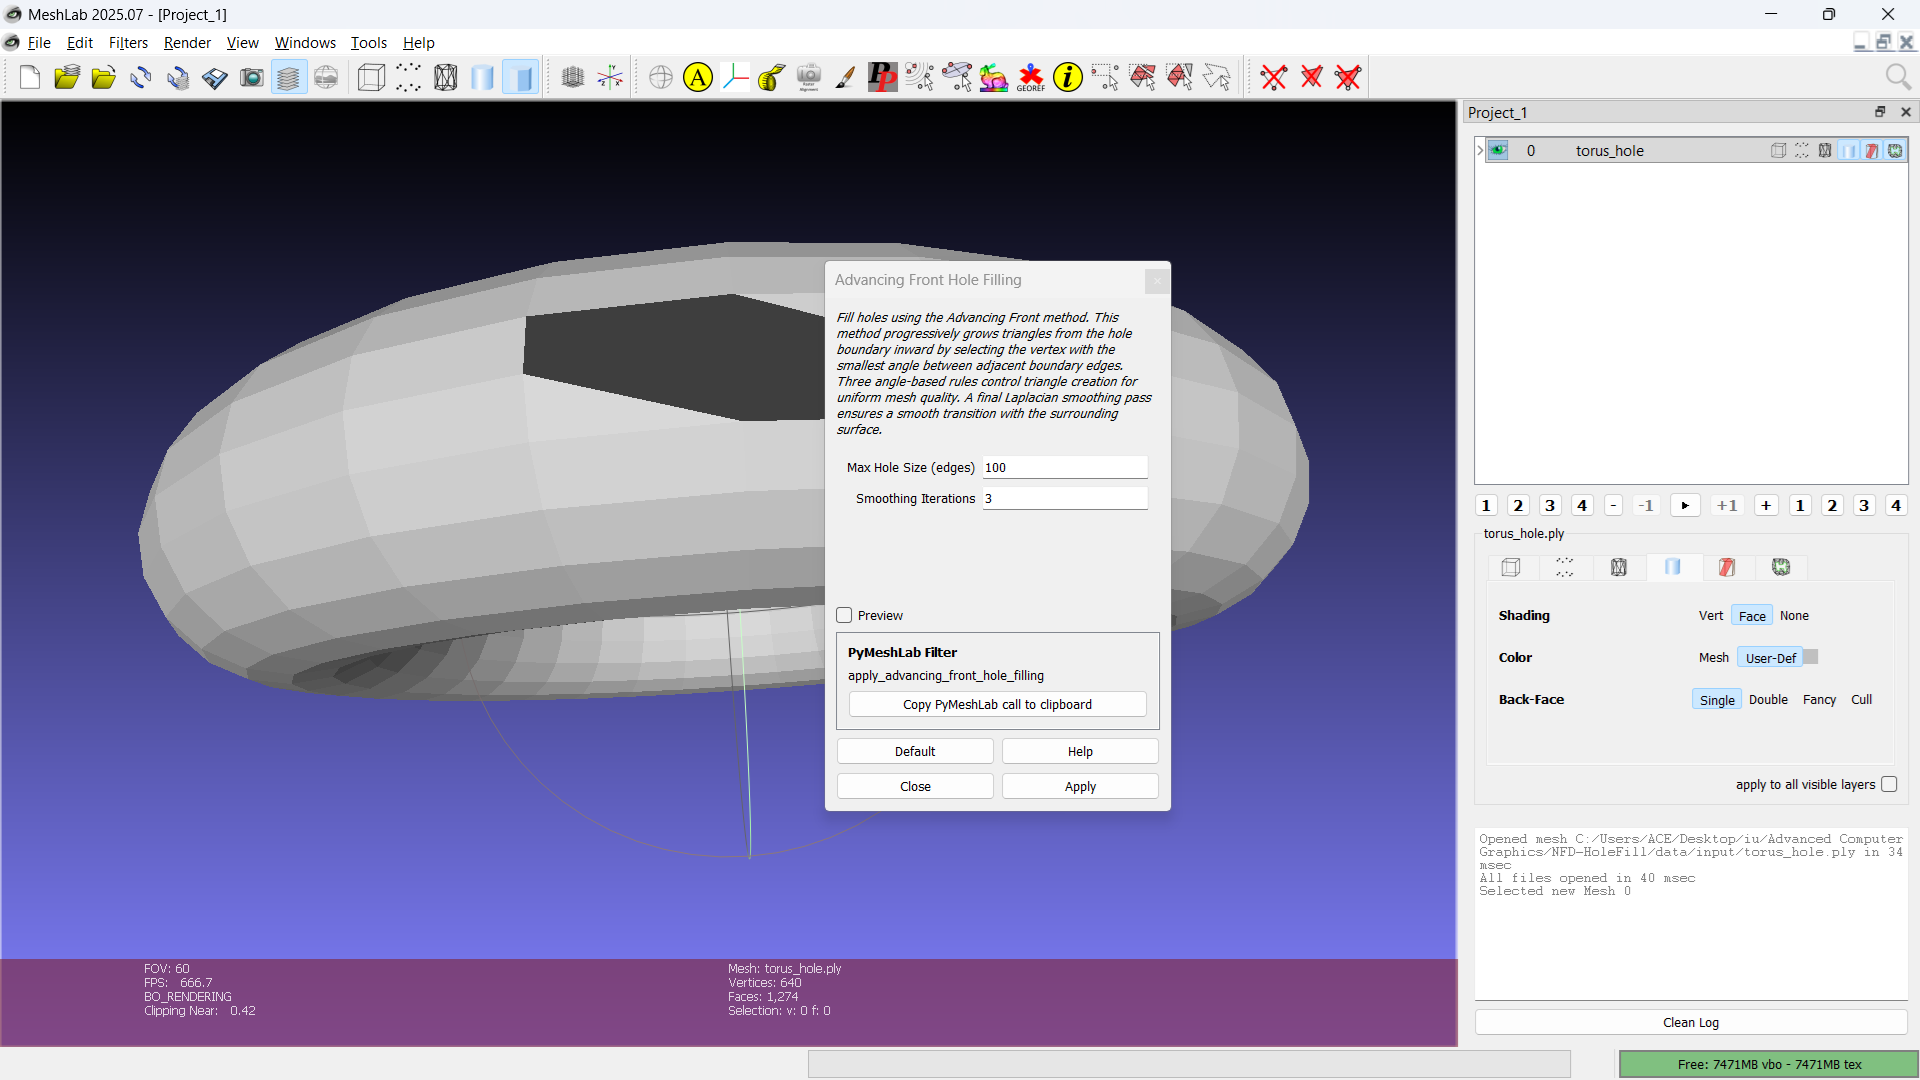
\includegraphics[width=0.55\textwidth]{03_filter_dialog.png}
\caption{Plugin parameter dialog in MeshLab.}
\label{fig:filter_dialog}
\end{figure}

\begin{figure}[H]
\centering
\begin{subfigure}[b]{0.48\textwidth}
  \centering
  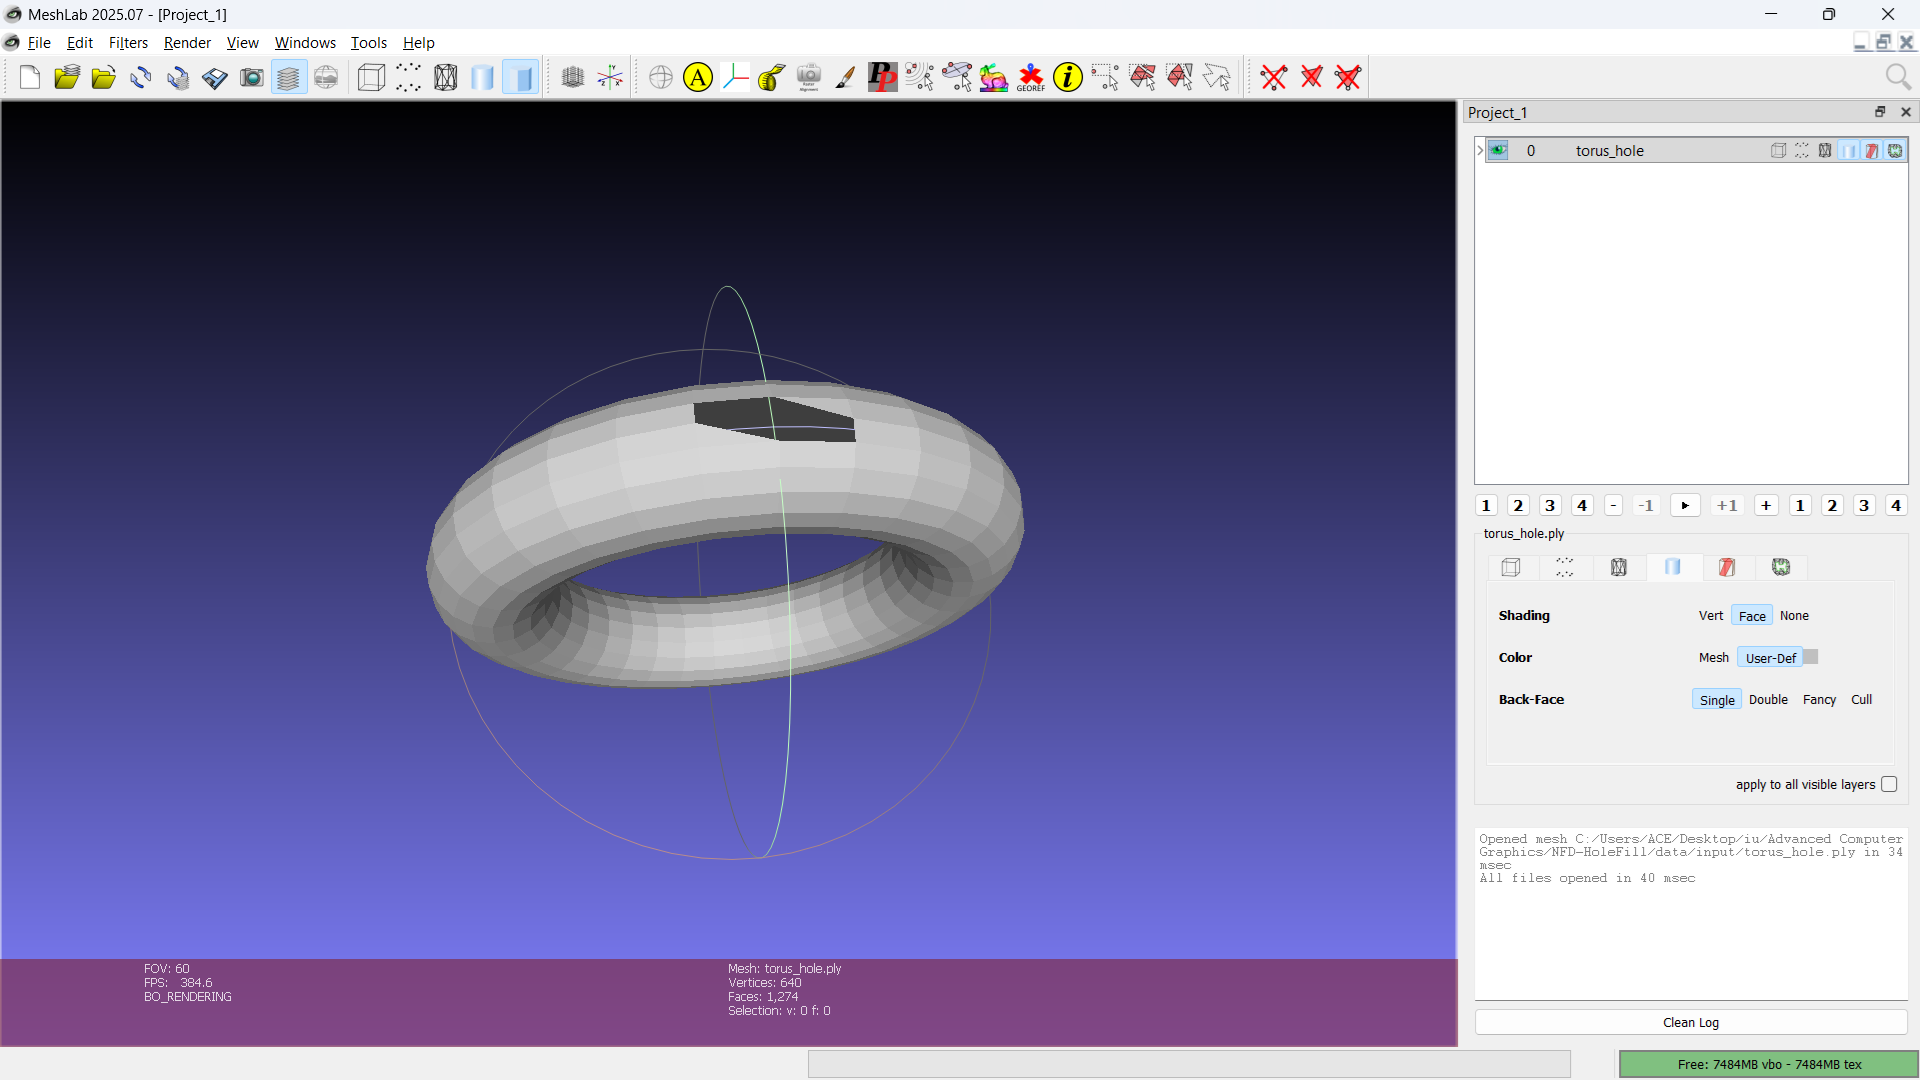
\includegraphics[width=\textwidth]{01_torus_with_hole.png}
  \caption{Before: torus with hole}
\end{subfigure}
\hfill
\begin{subfigure}[b]{0.48\textwidth}
  \centering
  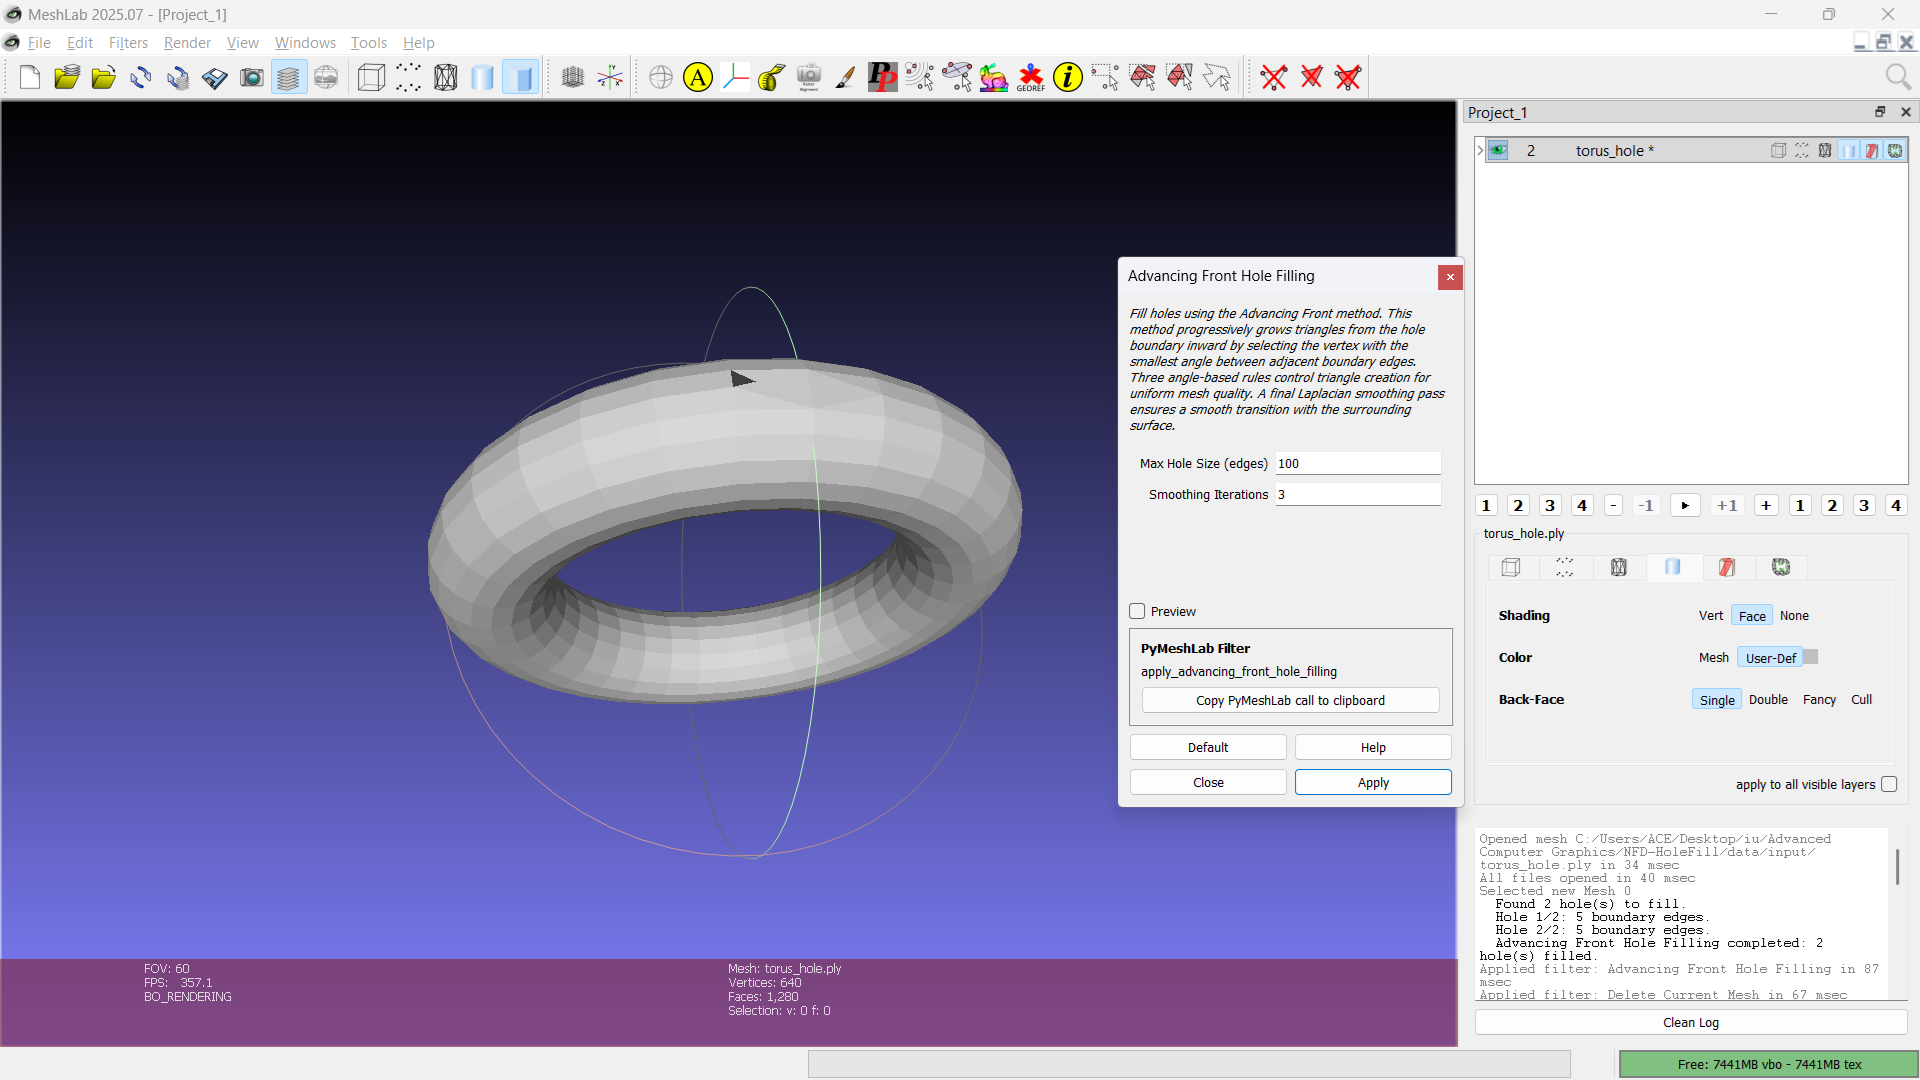
\includegraphics[width=\textwidth]{04_torus_filled.png}
  \caption{After: hole filled}
\end{subfigure}
\caption{Torus hole filling result (overview).}
\label{fig:torus_result}
\end{figure}

\begin{figure}[H]
\centering
\begin{subfigure}[b]{0.48\textwidth}
  \centering
  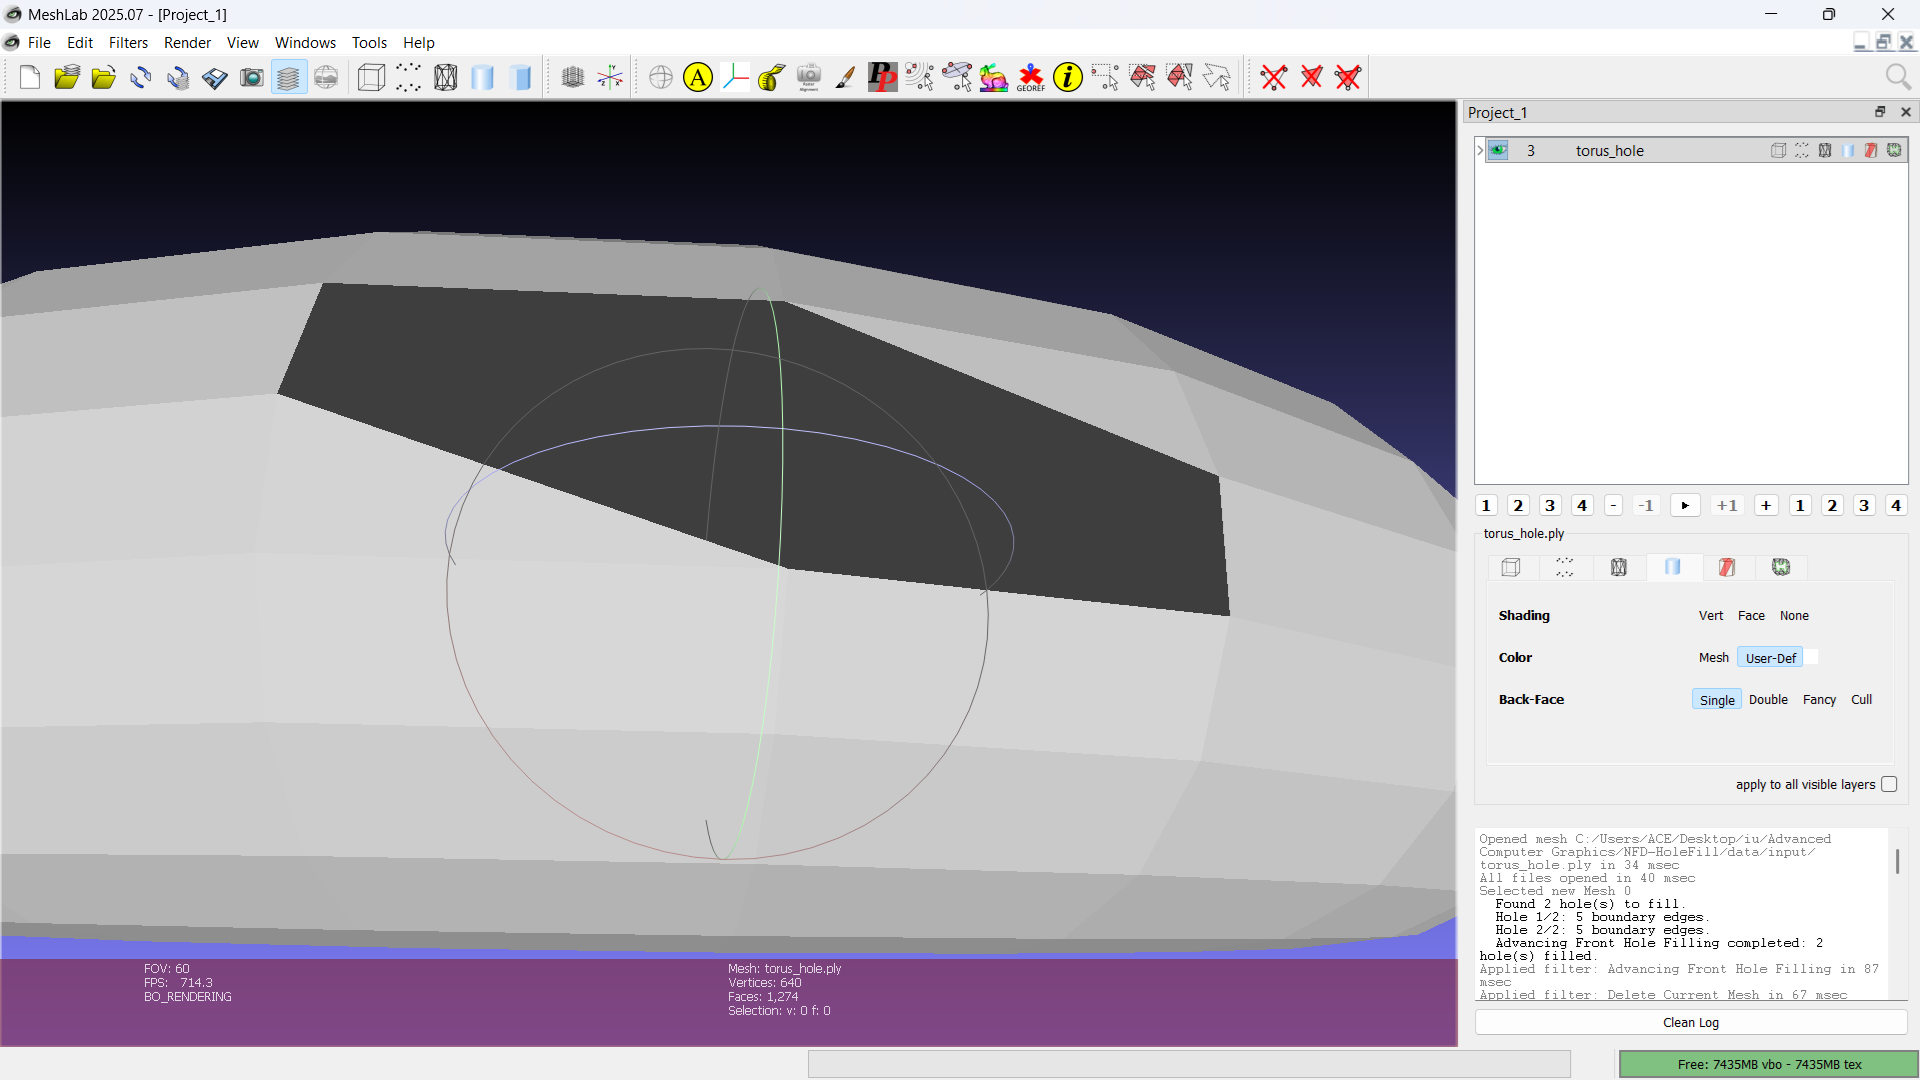
\includegraphics[width=\textwidth]{02_torus_closeup.png}
  \caption{Before: close-up of hole}
\end{subfigure}
\hfill
\begin{subfigure}[b]{0.48\textwidth}
  \centering
  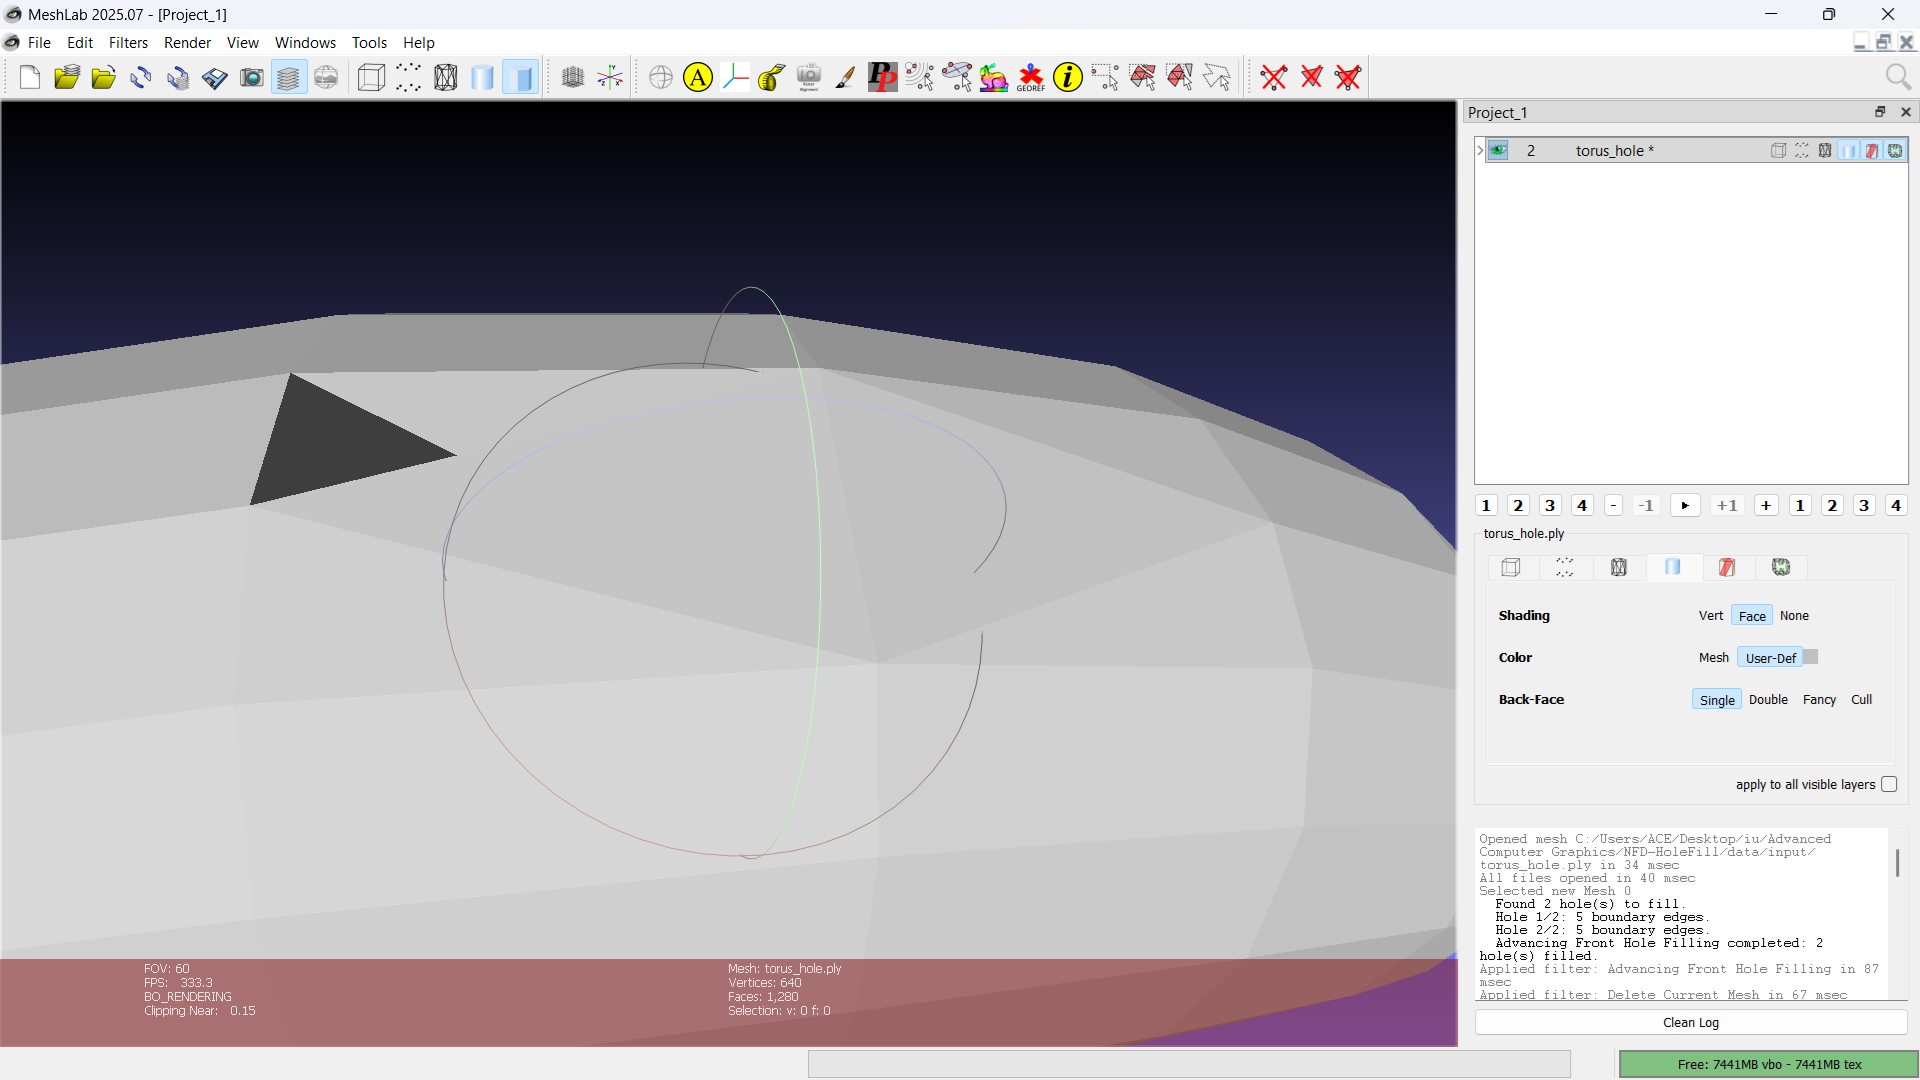
\includegraphics[width=\textwidth]{05_torus_filled_closeup.png}
  \caption{After: close-up of filled region}
\end{subfigure}
\caption{Torus hole filling result (close-up). The generated triangles blend smoothly with the surrounding mesh after Laplacian smoothing.}
\label{fig:torus_result_closeup}
\end{figure}

% ── Sphere ──
\subsection{Sphere Mesh (Large Hole)}

The plugin was also tested on a sphere with a larger hole to evaluate performance on wider gaps where Rules~2 and~3 are more frequently applied.

\begin{figure}[H]
\centering
\begin{subfigure}[b]{0.48\textwidth}
  \centering
  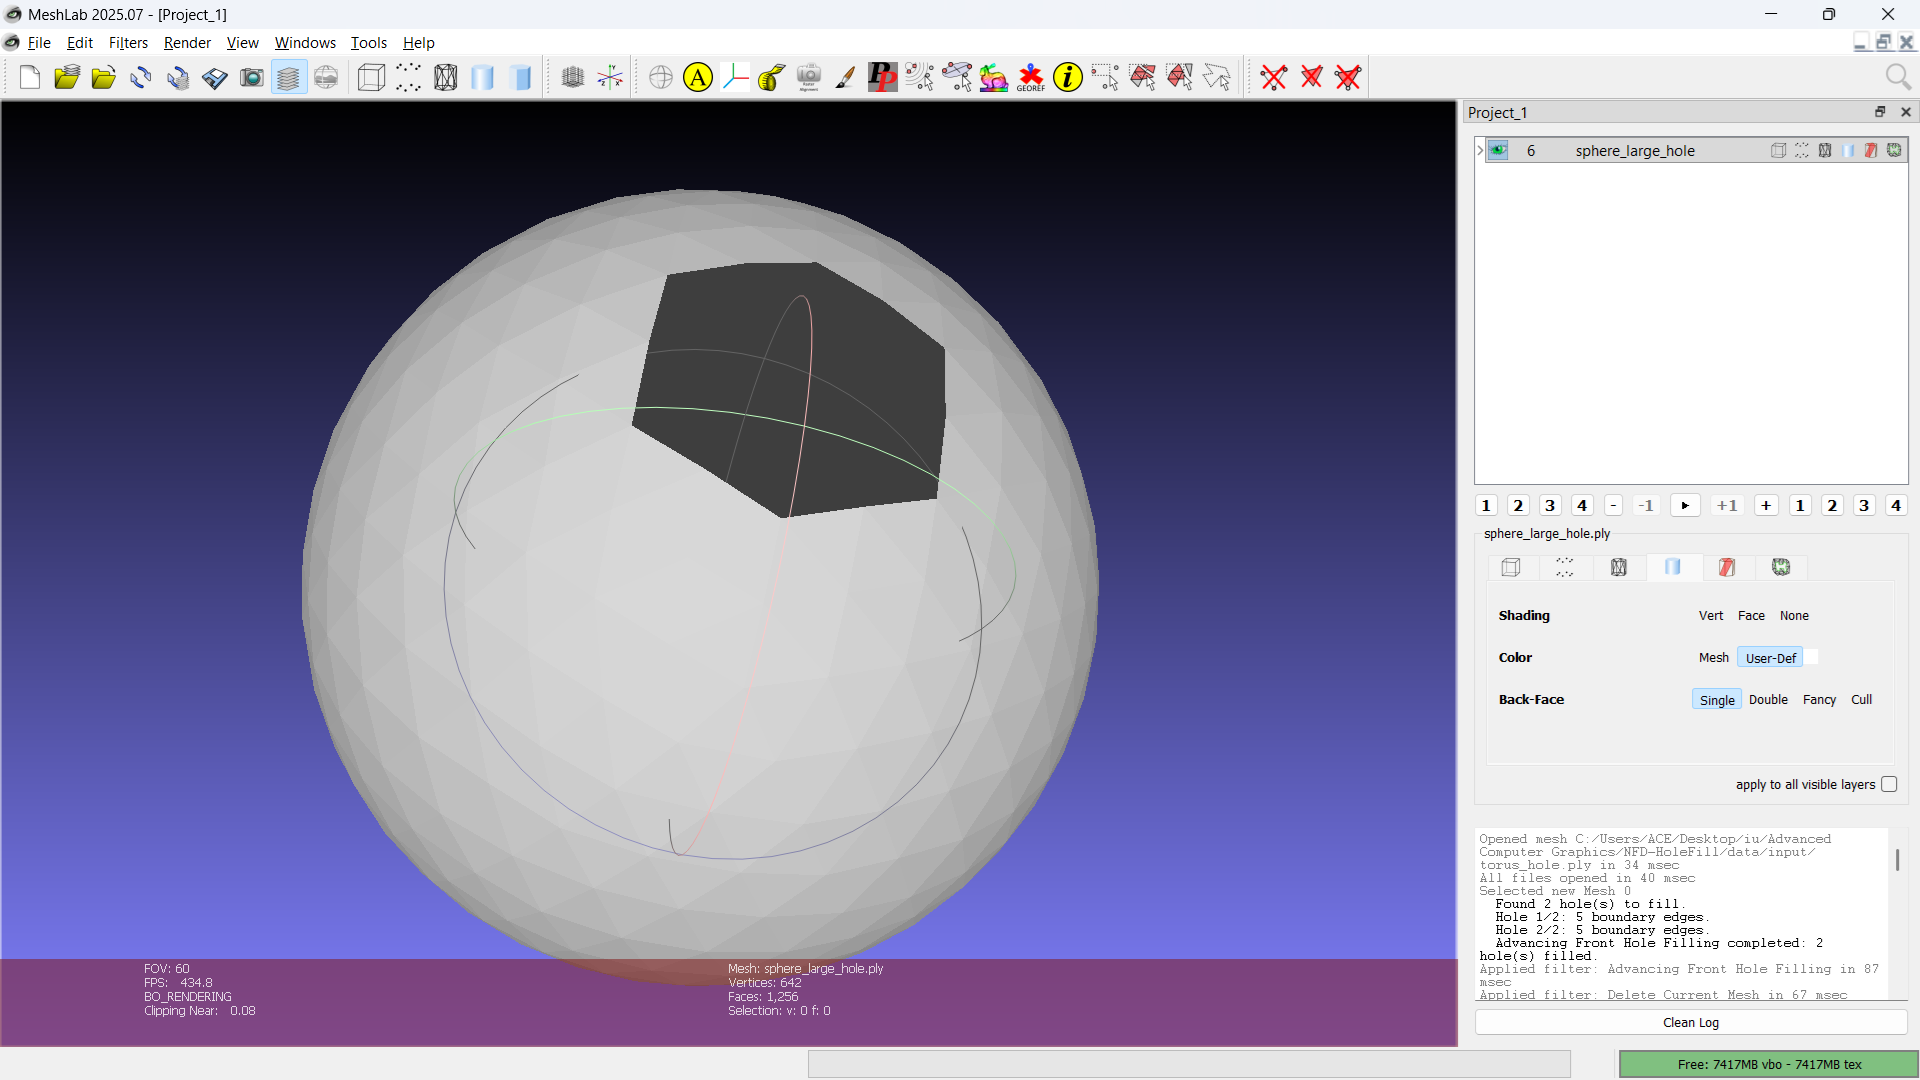
\includegraphics[width=\textwidth]{06_sphere_before.png}
  \caption{Before: sphere with large hole}
\end{subfigure}
\hfill
\begin{subfigure}[b]{0.48\textwidth}
  \centering
  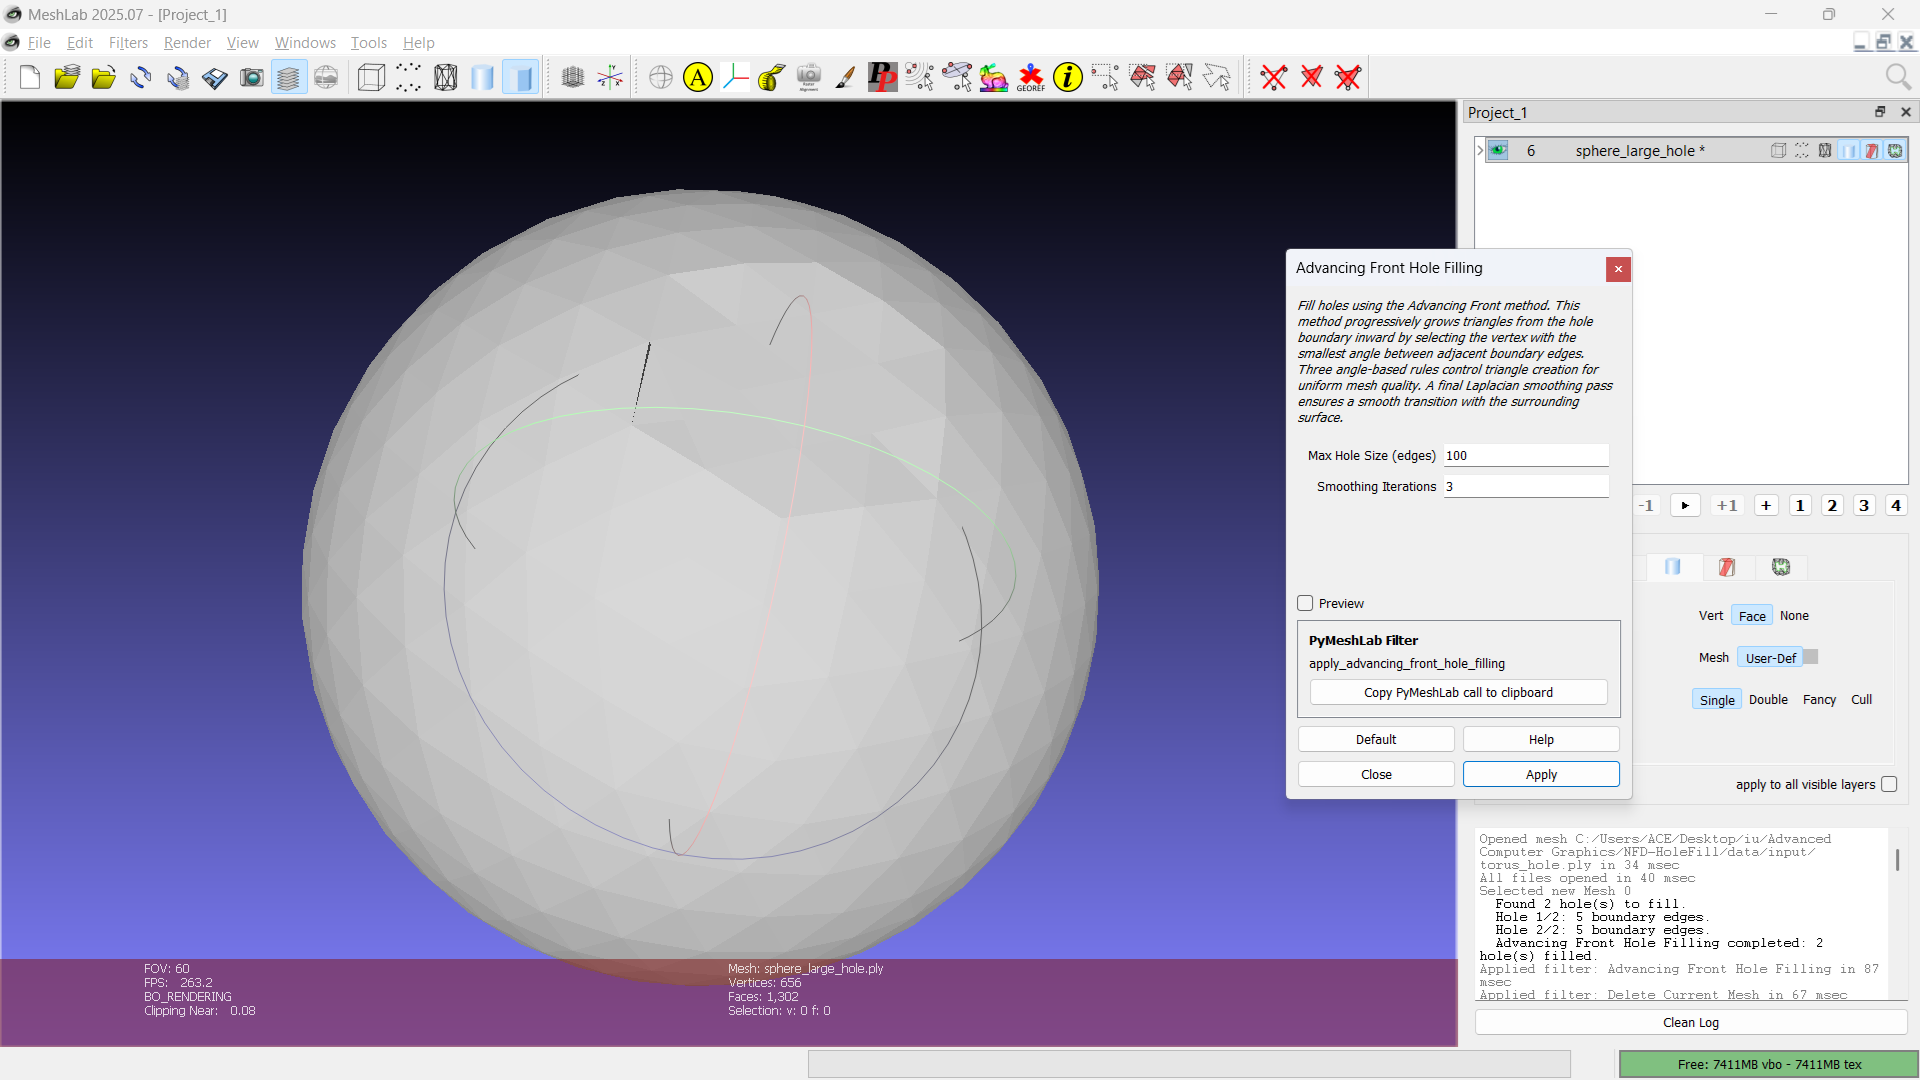
\includegraphics[width=\textwidth]{07_sphere_after.png}
  \caption{After: hole filled}
\end{subfigure}
\caption{Sphere large hole filling. The advancing front method produces uniform triangles even for larger holes by combining all three angle-based rules.}
\label{fig:sphere_result}
\end{figure}

% ============================================================
\section{Implementation}
% ============================================================

\subsection{Tools and Libraries}

\begin{table}[h]
\centering
\begin{tabular}{@{}lll@{}}
\toprule
\textbf{Component} & \textbf{Tool/Library} & \textbf{Purpose} \\
\midrule
C++ Framework & VCG Library & Mesh data structures, topology, normals \\
GUI/Plugin    & Qt 5.15     & MeshLab plugin interface \\
Build System  & CMake + Ninja & Cross-platform build \\
\bottomrule
\end{tabular}
\end{table}

\subsection{Plugin Structure}

\begin{itemize}[leftmargin=2em]
  \item \textbf{filter\_advancing\_front.h} -- Class declaration with \texttt{HoleBoundary} and \texttt{PatchMesh} data structures.
  \item \textbf{filter\_advancing\_front.cpp} -- Full algorithm implementation ($\sim$350 lines): \texttt{detectHoles()}, \texttt{advancingFrontFill()}, \texttt{smoothPatch()}, \texttt{mergePatchIntoMesh()}.
  \item \textbf{CMakeLists.txt} -- Build configuration via \texttt{add\_meshlab\_plugin()}.
\end{itemize}

\subsection{Parameters}

\begin{table}[h]
\centering
\begin{tabular}{@{}llcl@{}}
\toprule
\textbf{Parameter} & \textbf{Type} & \textbf{Default} & \textbf{Description} \\
\midrule
MaxHoleSize        & int  & 100 & Max boundary edges per hole \\
SmoothingIterations & int & 3   & Laplacian smoothing passes \\
\bottomrule
\end{tabular}
\end{table}

\subsection{Key Implementation Details}

\paragraph{Ocf Components.}
CMeshO uses VCG's Optional Component Framework (Ocf) for face--face and vertex--face adjacency. These must be explicitly enabled before topology operations via \texttt{m.face.EnableFFAdjacency()}, \texttt{m.face.EnableVFAdjacency()}, and \texttt{m.vert.EnableVFAdjacency()}. Omitting this causes a runtime exception.

\paragraph{Front Data Structure.}
The active front is a \texttt{std::vector<int>} of vertex indices. Boundary vertices occupy indices $0 \dots n{-}1$; new interior vertices are appended. Rule~1 erases one element, Rule~2 replaces one, and Rule~3 replaces one and inserts one.

\paragraph{Average Edge Length.}
$L_{\text{avg}}$ is computed once from the original boundary and used consistently for all new vertex placements, ensuring generated triangles match the surrounding mesh resolution.

% ============================================================
\section{How to Build and Run}
% ============================================================

\begin{enumerate}[leftmargin=2em]
  \item Place plugin files in \texttt{meshlab-src/src/meshlabplugins/filter\_advancing\_front/}
  \item Register the plugin in \texttt{meshlab-src/src/CMakeLists.txt}
  \item Set up VS environment: \texttt{call vcvarsall.bat x64}
  \item Build: \texttt{cmake --build build2 --target filter\_advancing\_front}
  \item Run: \texttt{build2/src/distrib/meshlab.exe}
  \item Import a mesh with holes, apply \texttt{Filters > Remeshing > Advancing Front Hole Filling}
\end{enumerate}

See \texttt{BUILD\_AND\_RUN.md} for detailed instructions.

% ============================================================
\section{Conclusion}
% ============================================================

This assignment implements the Advancing Front hole filling algorithm as a MeshLab C++ plugin. The method uses three angle-based rules to progressively grow triangles from the boundary inward, producing well-shaped meshes with uniform triangle quality. The angle-based vertex selection ensures that narrow gaps are closed first, preventing self-intersection and maintaining good aspect ratios. Combined with Laplacian smoothing, the result is a smooth, seamless patch that blends naturally with the surrounding surface geometry. The results on both torus and sphere meshes demonstrate that the method handles holes of varying sizes and curvatures effectively.

% ============================================================
\begin{thebibliography}{9}

\bibitem{liepa2003}
P.~Liepa, ``Filling holes in meshes,'' in \textit{Proc.\ Eurographics Symposium on Geometry Processing}, pp.~200--205, 2003.

\bibitem{zhao2007}
W.~Zhao, S.~Gao, and H.~Lin, ``A robust hole-filling algorithm for triangular mesh,'' \textit{The Visual Computer}, vol.~23, no.~12, pp.~987--997, 2007.

\bibitem{lo1985}
S.~H.~Lo, ``A new mesh generation scheme for arbitrary planar domains,'' \textit{International Journal for Numerical Methods in Engineering}, vol.~21, no.~8, pp.~1403--1426, 1985.

\end{thebibliography}

\end{document}
